Carrier Sense Multiple Access with Enhanced Collision Avoidance (CSMA/ECA) achieves less collisions and outperforms CSMA/CA in most typical scenarios. This is done by choosing a deterministic backoff after each successful transmission. Its evolution, CSMA/E2CA introduces stickiness in the process in order to shorten the convergence time towards a collision-free state by setting a number of occasions a deterministic backoff is used after each successful transmission~\cite{CSMA_ECA} .

Stickiness can reduce the convergence time by orders of magnitude when the number of contenders $\eta$ is less or equal than the system capacity $C$ as defined in Eq.~\ref{eq:capacity}, where $\lceil{\cdotp}\rceil$ is the ceiling operator, $E[\cdotp]$ is the expectation operator, $\mathcal{U}$ is the uniform distribution and $CW_{min}$ is the minimum contention window of the system (usually $CW_{min}=32$ for 802.11 networks). 

\begin{equation} \label{eq:capacity}	
	C = \lceil{E[\mathcal{U}[0, CW_{min} - 1]]}\rceil
\end{equation}

\begin{figure}[htbp]
  \centering
%   \psfrag{psfrag1}[Bc][Bc][0.9]{$\eta$}
  \includegraphics[width=0.7\linewidth, angle = -90]{figures/throughput/throughput.eps}
  \caption{Throughput and how it is affected when $\eta > C$
  \label{fig:throughput}}
\end{figure}

The system capacity $C$ in turn refers to the time slots available for transmission in the schedule. 

%As can be appreciated in Figure~\ref{fig:throughput}, the constraint $\eta \leq C$ is also limiting the throughput in CSMA/E2CA.

In Figure~\ref{fig:throughput}, when $\eta > C$ the CSMA/E2CA system is overcrowded with contenders and the collision-free state is compromised. As more contenders are introduced, the system behavior tends to be more like CSMA/CA: nodes are forced to choose a random backoff.

In this work, a fully-distributed version of CSMA/E2CA is presented and the throughput issue when $\eta > C$ is assessed using Fair Share.